\documentclass[12pt,a4paper]{article}
\usepackage[utf8]{inputenc}
\usepackage{pdfpages}
\usepackage[magyar]{babel}
\usepackage{hyperref}	
\hypersetup{					
colorlinks=false,						
pdfborder={0 0 0},
}
\usepackage{fancyhdr}
\usepackage[left=2cm,right=2cm,top=3.5cm,bottom=3cm,headsep=50pt]{geometry}

\begin{document}
%=================================================
\thispagestyle{empty}
\begin{center}

\includegraphics[scale=0.3]{bme.pdf}\\
\large{Budapesti Műszaki- és Gazdaságtudományi Egyetem\\
Gépészmérnöki kar}\\[1cm]
\begin{Huge}
\textbf{Mechatronika projekt}
\end{Huge}\\[0.5cm]

\Large{BMEGEFOAMM3}\\[2cm]
\Huge{\bf{3D szkenner}}\\[2.5cm]
\bf{\Large{Tar Dániel\\[5pt]
		Bognár Máté\\
		Varga Roland}}\\[1cm]


\includegraphics[scale=0.5]{mogilogo.jpg}\\[1cm]
\large{\today}
\end{center}
%=================================================
\newpage
\tableofcontents
\newpage
\pagestyle{fancy}
\fancyhf{}
\rhead{Tar Dániel\\Bognár Máté\\Varga Roland}
\lhead{3D szkenner}
\cfoot{\thepage. oldal}
%=================================================
\section{Feladat leírása}
%=================================================
\section{Alapul vett szakirodalom}
Ide jönne a két nagyon hasonló projekt meghivatkozva!
%=================================================
\section{Felhasznált hardverek}
\subsection{Beszerzett eszközök}
A projektfeladat már az előző évben is ki volt adva, a tavalyi csoportnak ugyan nem sikerült befejeznie, de néhány általuk készített alkatrész öröklődött. Így már kézhez kaptuk egy  LFL650-5-12(9x20)60-as típusú vonallézert,
egy unipoláris léptető motort, a tanszéki KUTESZ alkatrészekből összeállított állvánnyal és egy kisebb méretű asztallal,
illetve a motor meghajtó áramkört is.
\\[10pt]
A felhasznált hardverek egy másik része Bojtos Attila tanár úrtól származik. Ilyen a fényképezőgép állvány, az erre később rögzített 20x20-as ITEM-5-ös profil, és egy Canyon márkájú, 640x480-as felbontású webkamera.
\\[10pt]
Általunk beszerzett alkatrész még a forgóasztalt vezérlő áramkör: ...
És a lézert kapcsoló egység: ...
 \begin{figure}[h!]
 	\centering
 	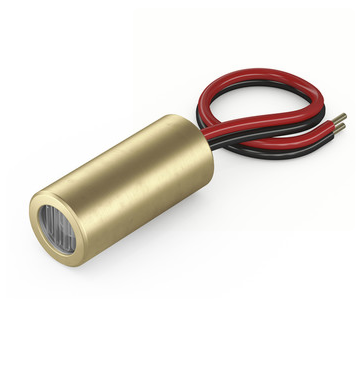
\includegraphics[scale=0.5]{images/laser}
 	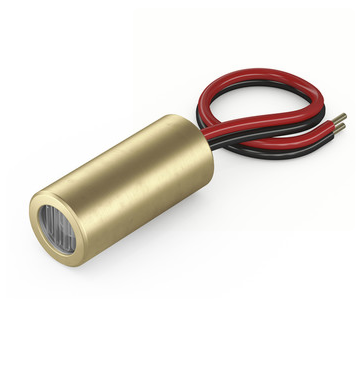
\includegraphics[scale=0.5]{images/laser}
	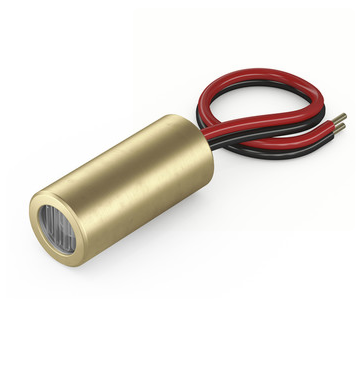
\includegraphics[scale=0.5]{images/laser}
	\caption{Beszerzett eszközök}
\end{figure}

\subsection{Saját készítésű eszközök}
Az általunk tervezett alkatrészek többsége 3D nyomtatással készült, ezek a kamerát és lézert az ITEM profilra rögzítő elemek. A lézer lefogó, amely a lézert rögzíti a profil közepén. És a kamera tartó, ami két alkatrész közé szorítja be a kamera alsó részét, a gyári foglalathoz hasonló módon.\\[10pt]
Emellett a követelményeknek megfelelő szkennelhető tárgyméret miatt tervezni kellett egy új forgóasztalt. Ez az asztal 180mm átmérőjű, központosító körökkel ellátott, a KUTESZ elemekkel kompatibilis furatkiosztású elem.
Végül a profilt a kamera állványra rögzítő elem egy 6mm vastag,  lemez alkatrész.
 \begin{figure}[h!]
 	\centering
	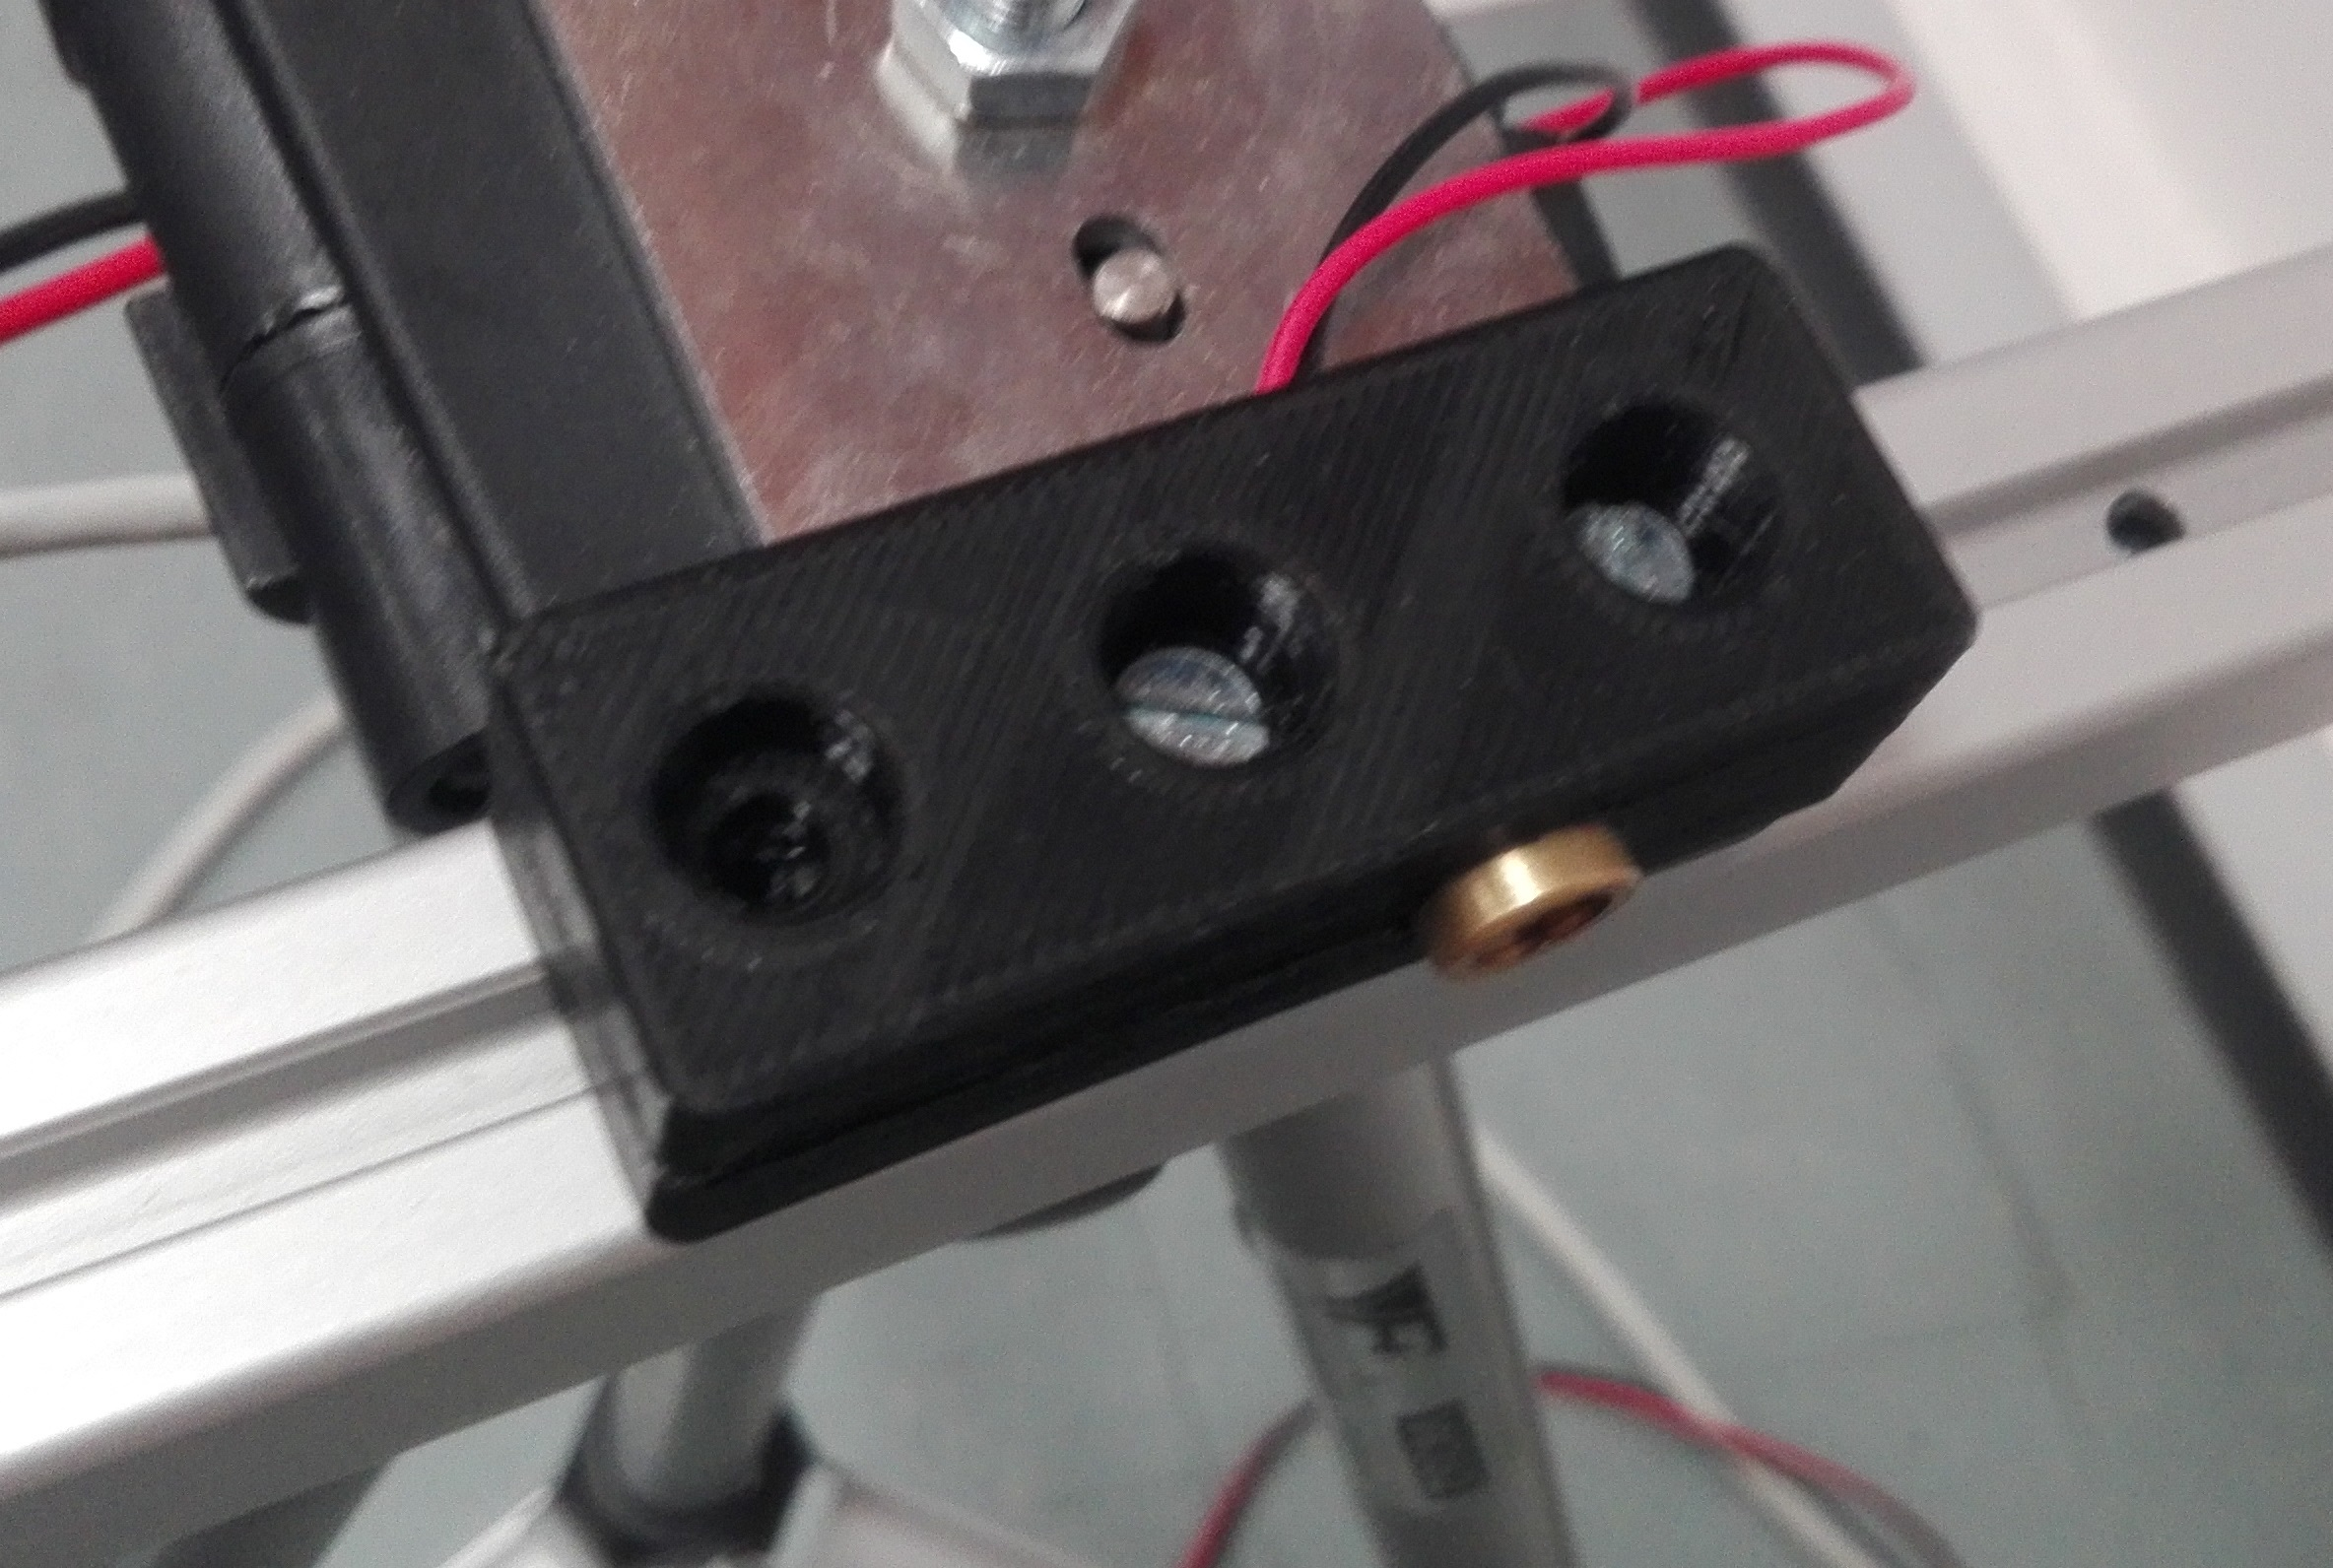
\includegraphics[height=5cm]{images/lezerlefogo}
	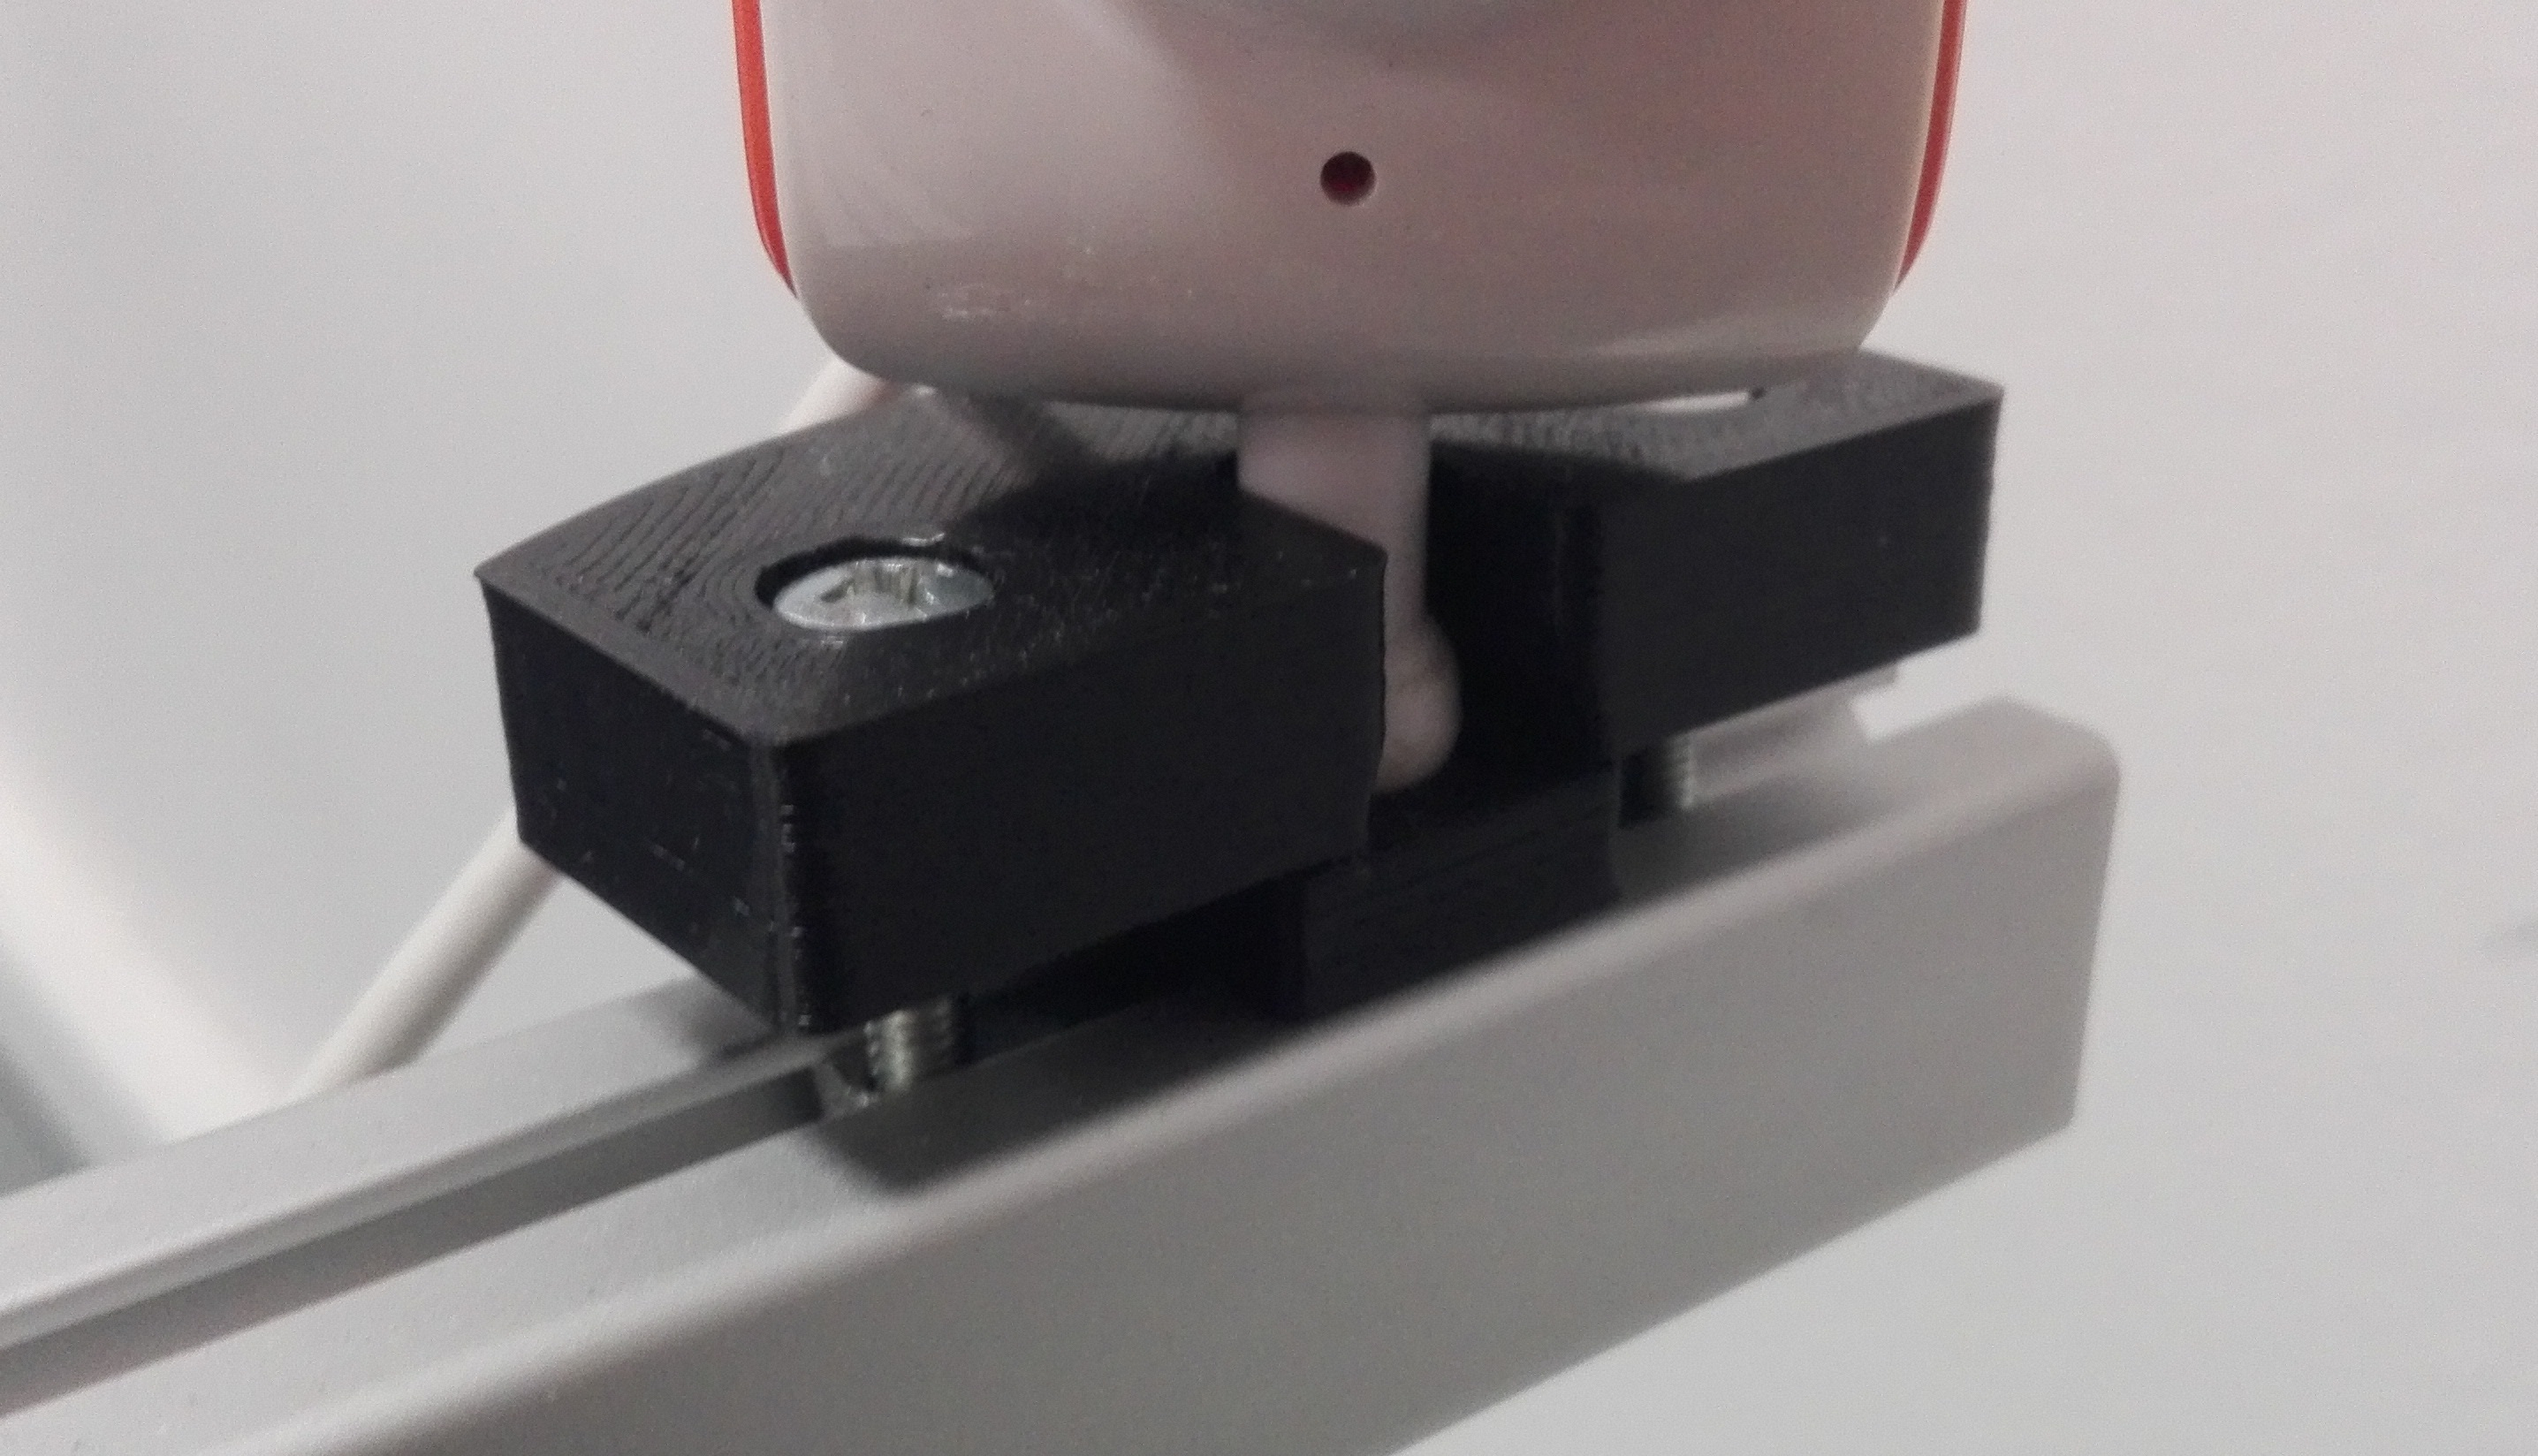
\includegraphics[height=5cm]{images/kameratarto}
	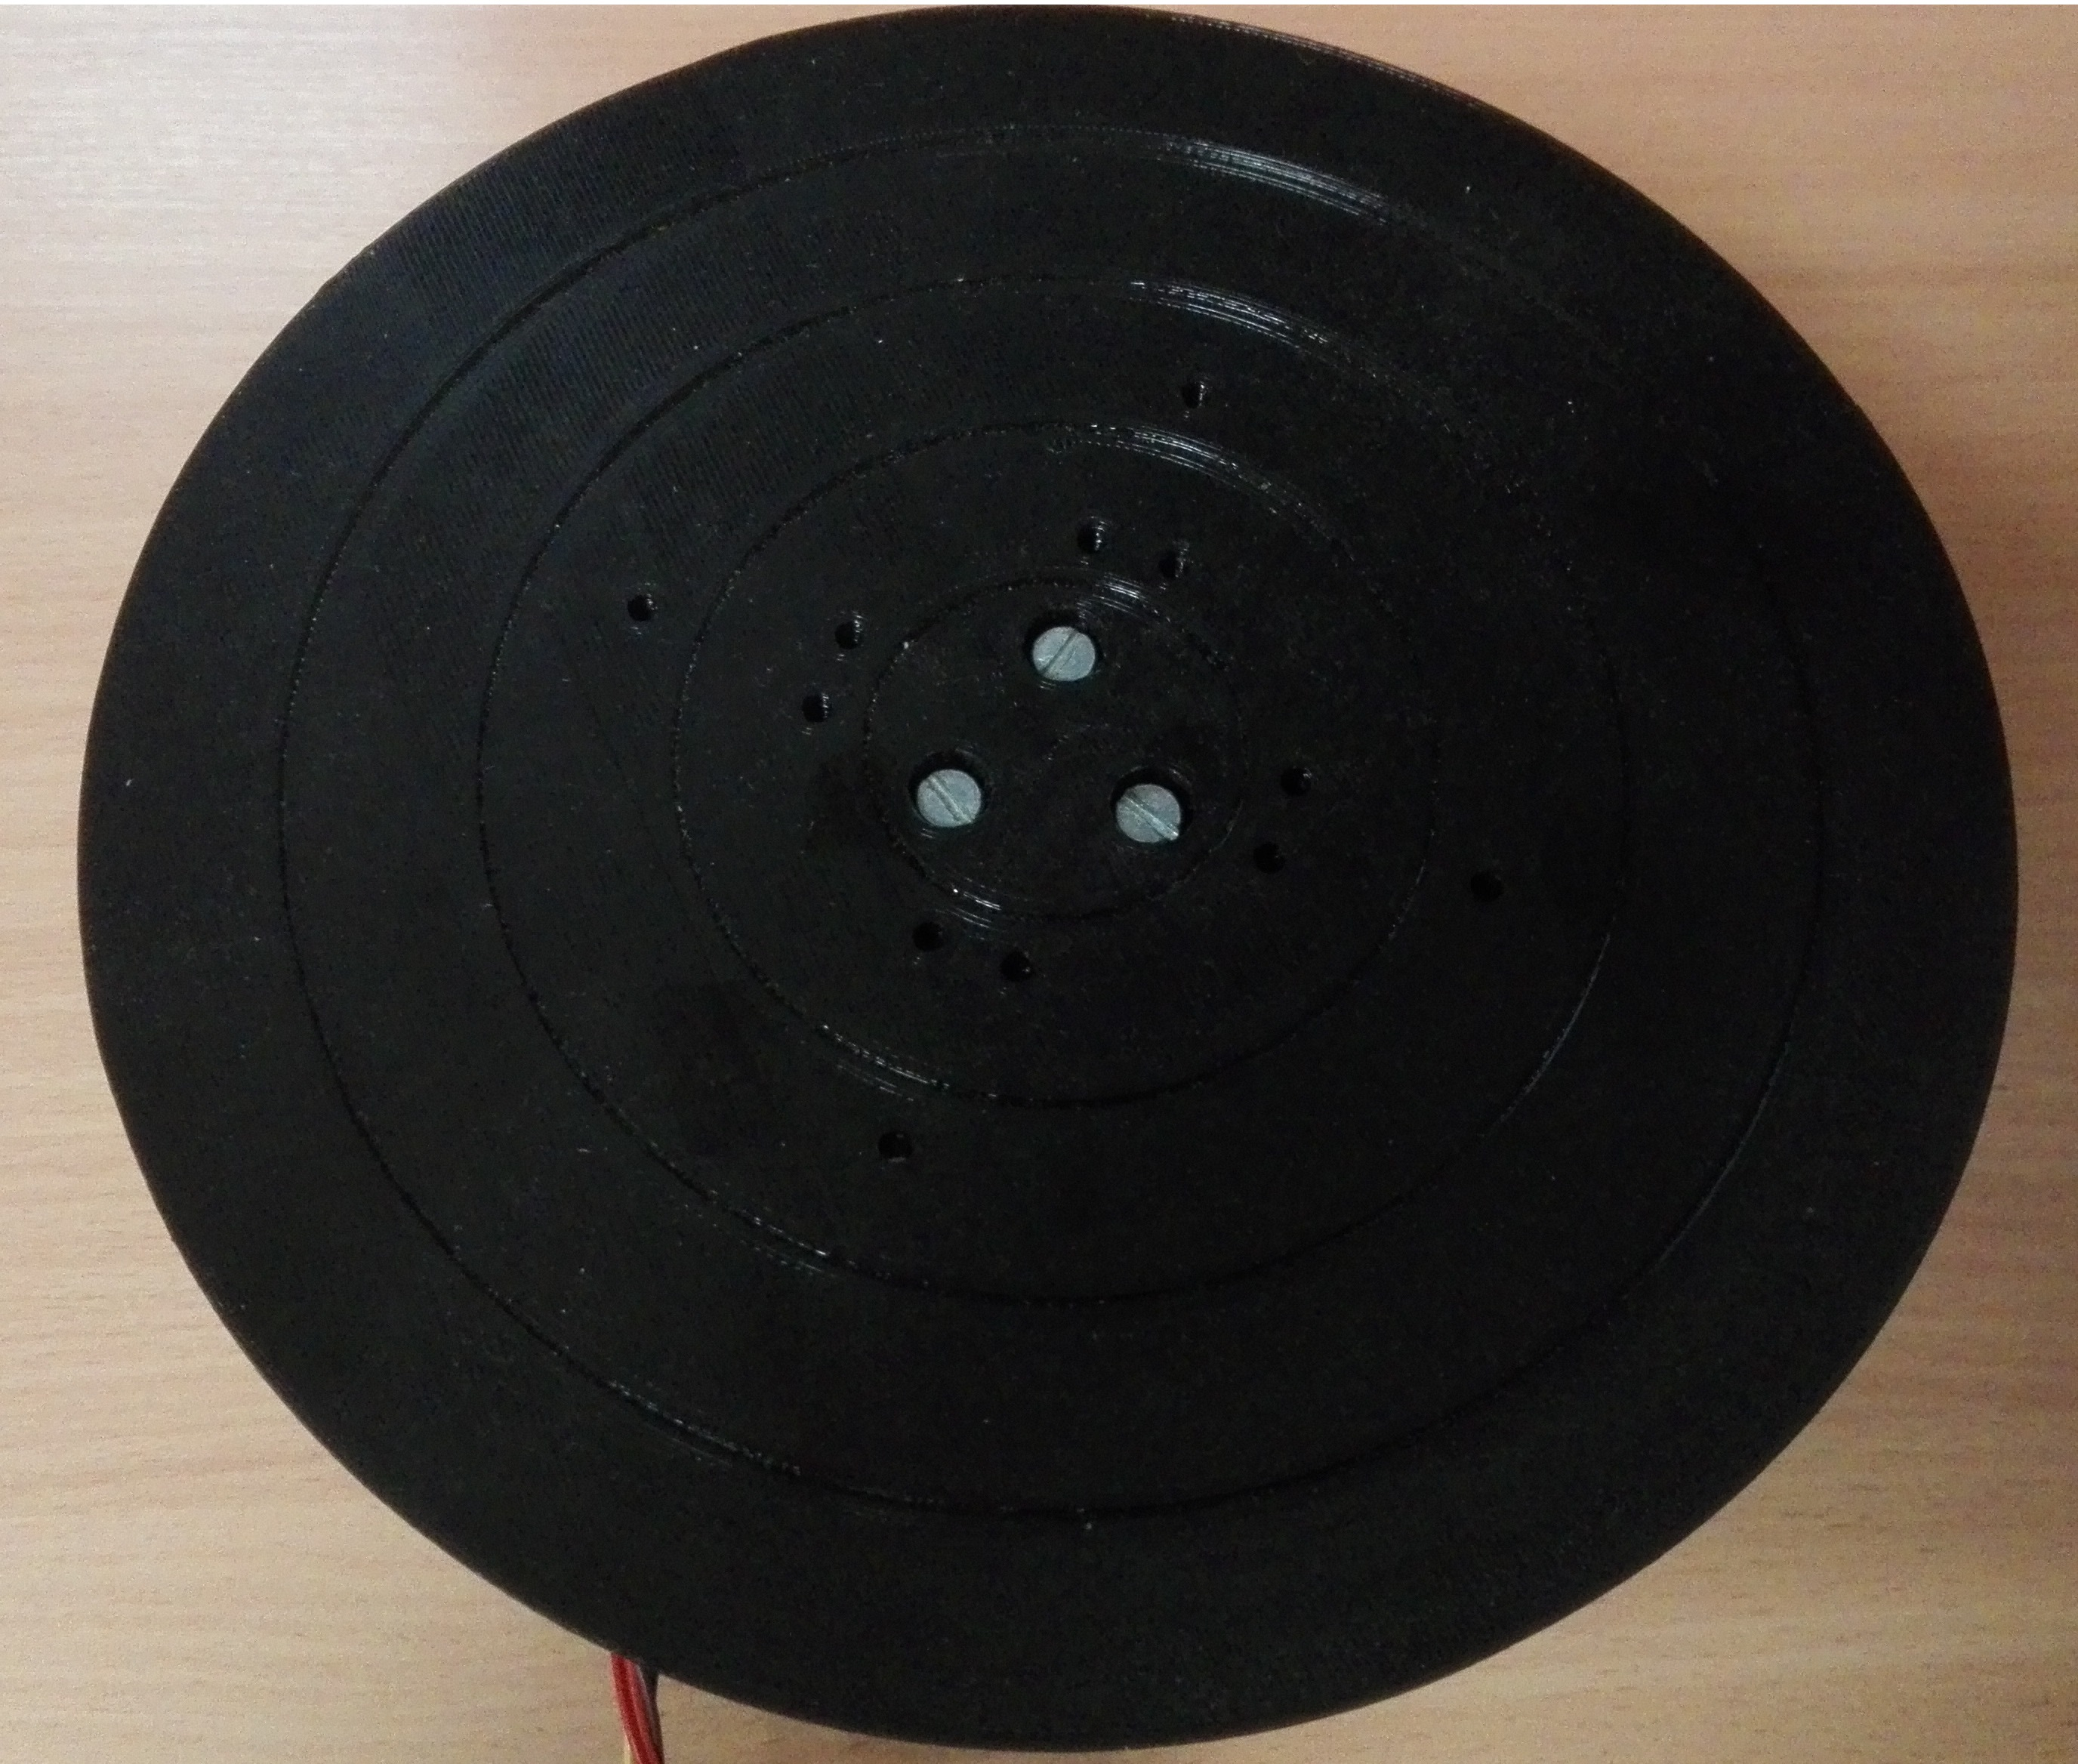
\includegraphics[height=5cm]{images/asztal}
	\caption{Saját készítésű eszközök}
\end{figure}
\subsection{Hardverek közötti csatlakozás}

Az elkészült konstrukció két részből áll. Az egyik a forgóasztal, a motor, a meghajtója és ennek vezérlő áramköre. A meghajtónak hálózati tápellátás szükséges, míg a vezérlő jelenleg számítógépről kapja az áramot USB-n keresztül.
\\[10pt]
A másik rész a kamera állvány, rajta a lézerrel és webkamerával. Utóbbi közvetlen csatlakozik a számítógéphez, míg a lézer az őt vezérlő arduino-n keresztül, szintén USB segítségével.\ref{kameraallvanyra}
\\[10pt]
Így a szkenner két részben hordozható kivitelű.\ref{hordozhatosag}
 \begin{figure}[h!]
	\centering
	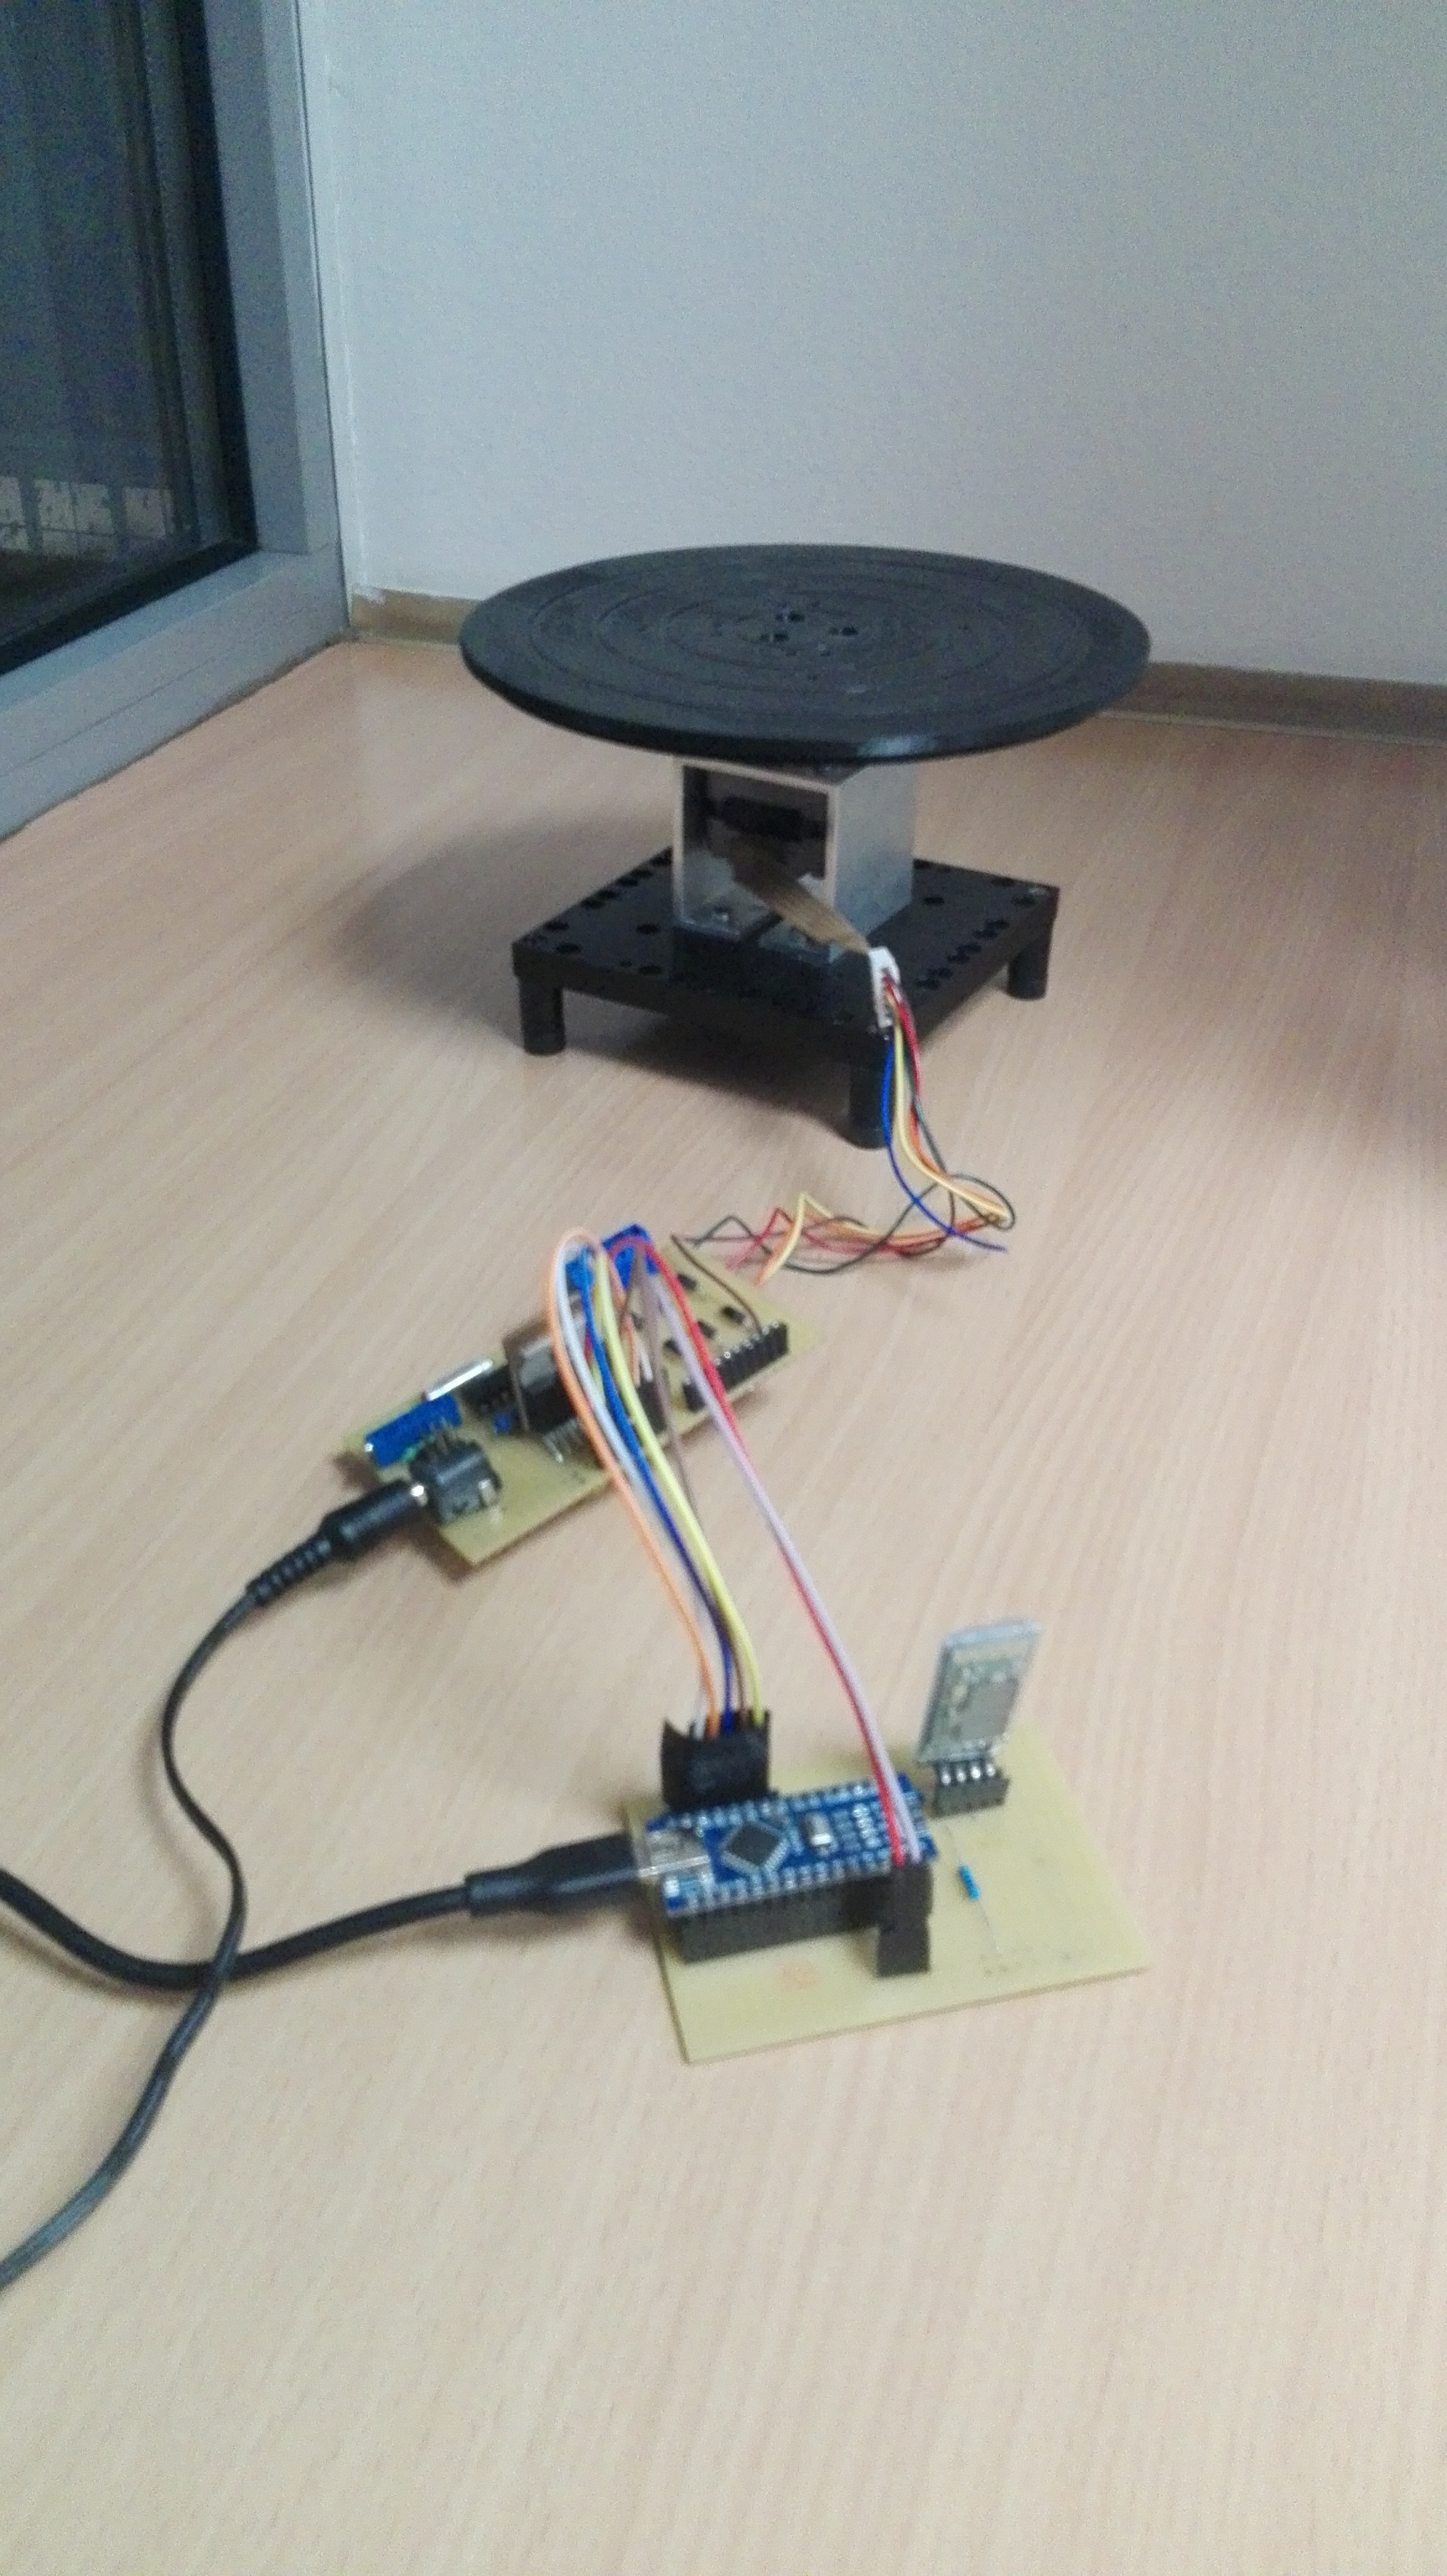
\includegraphics[width=5.5cm]{images/forgoasztal}
	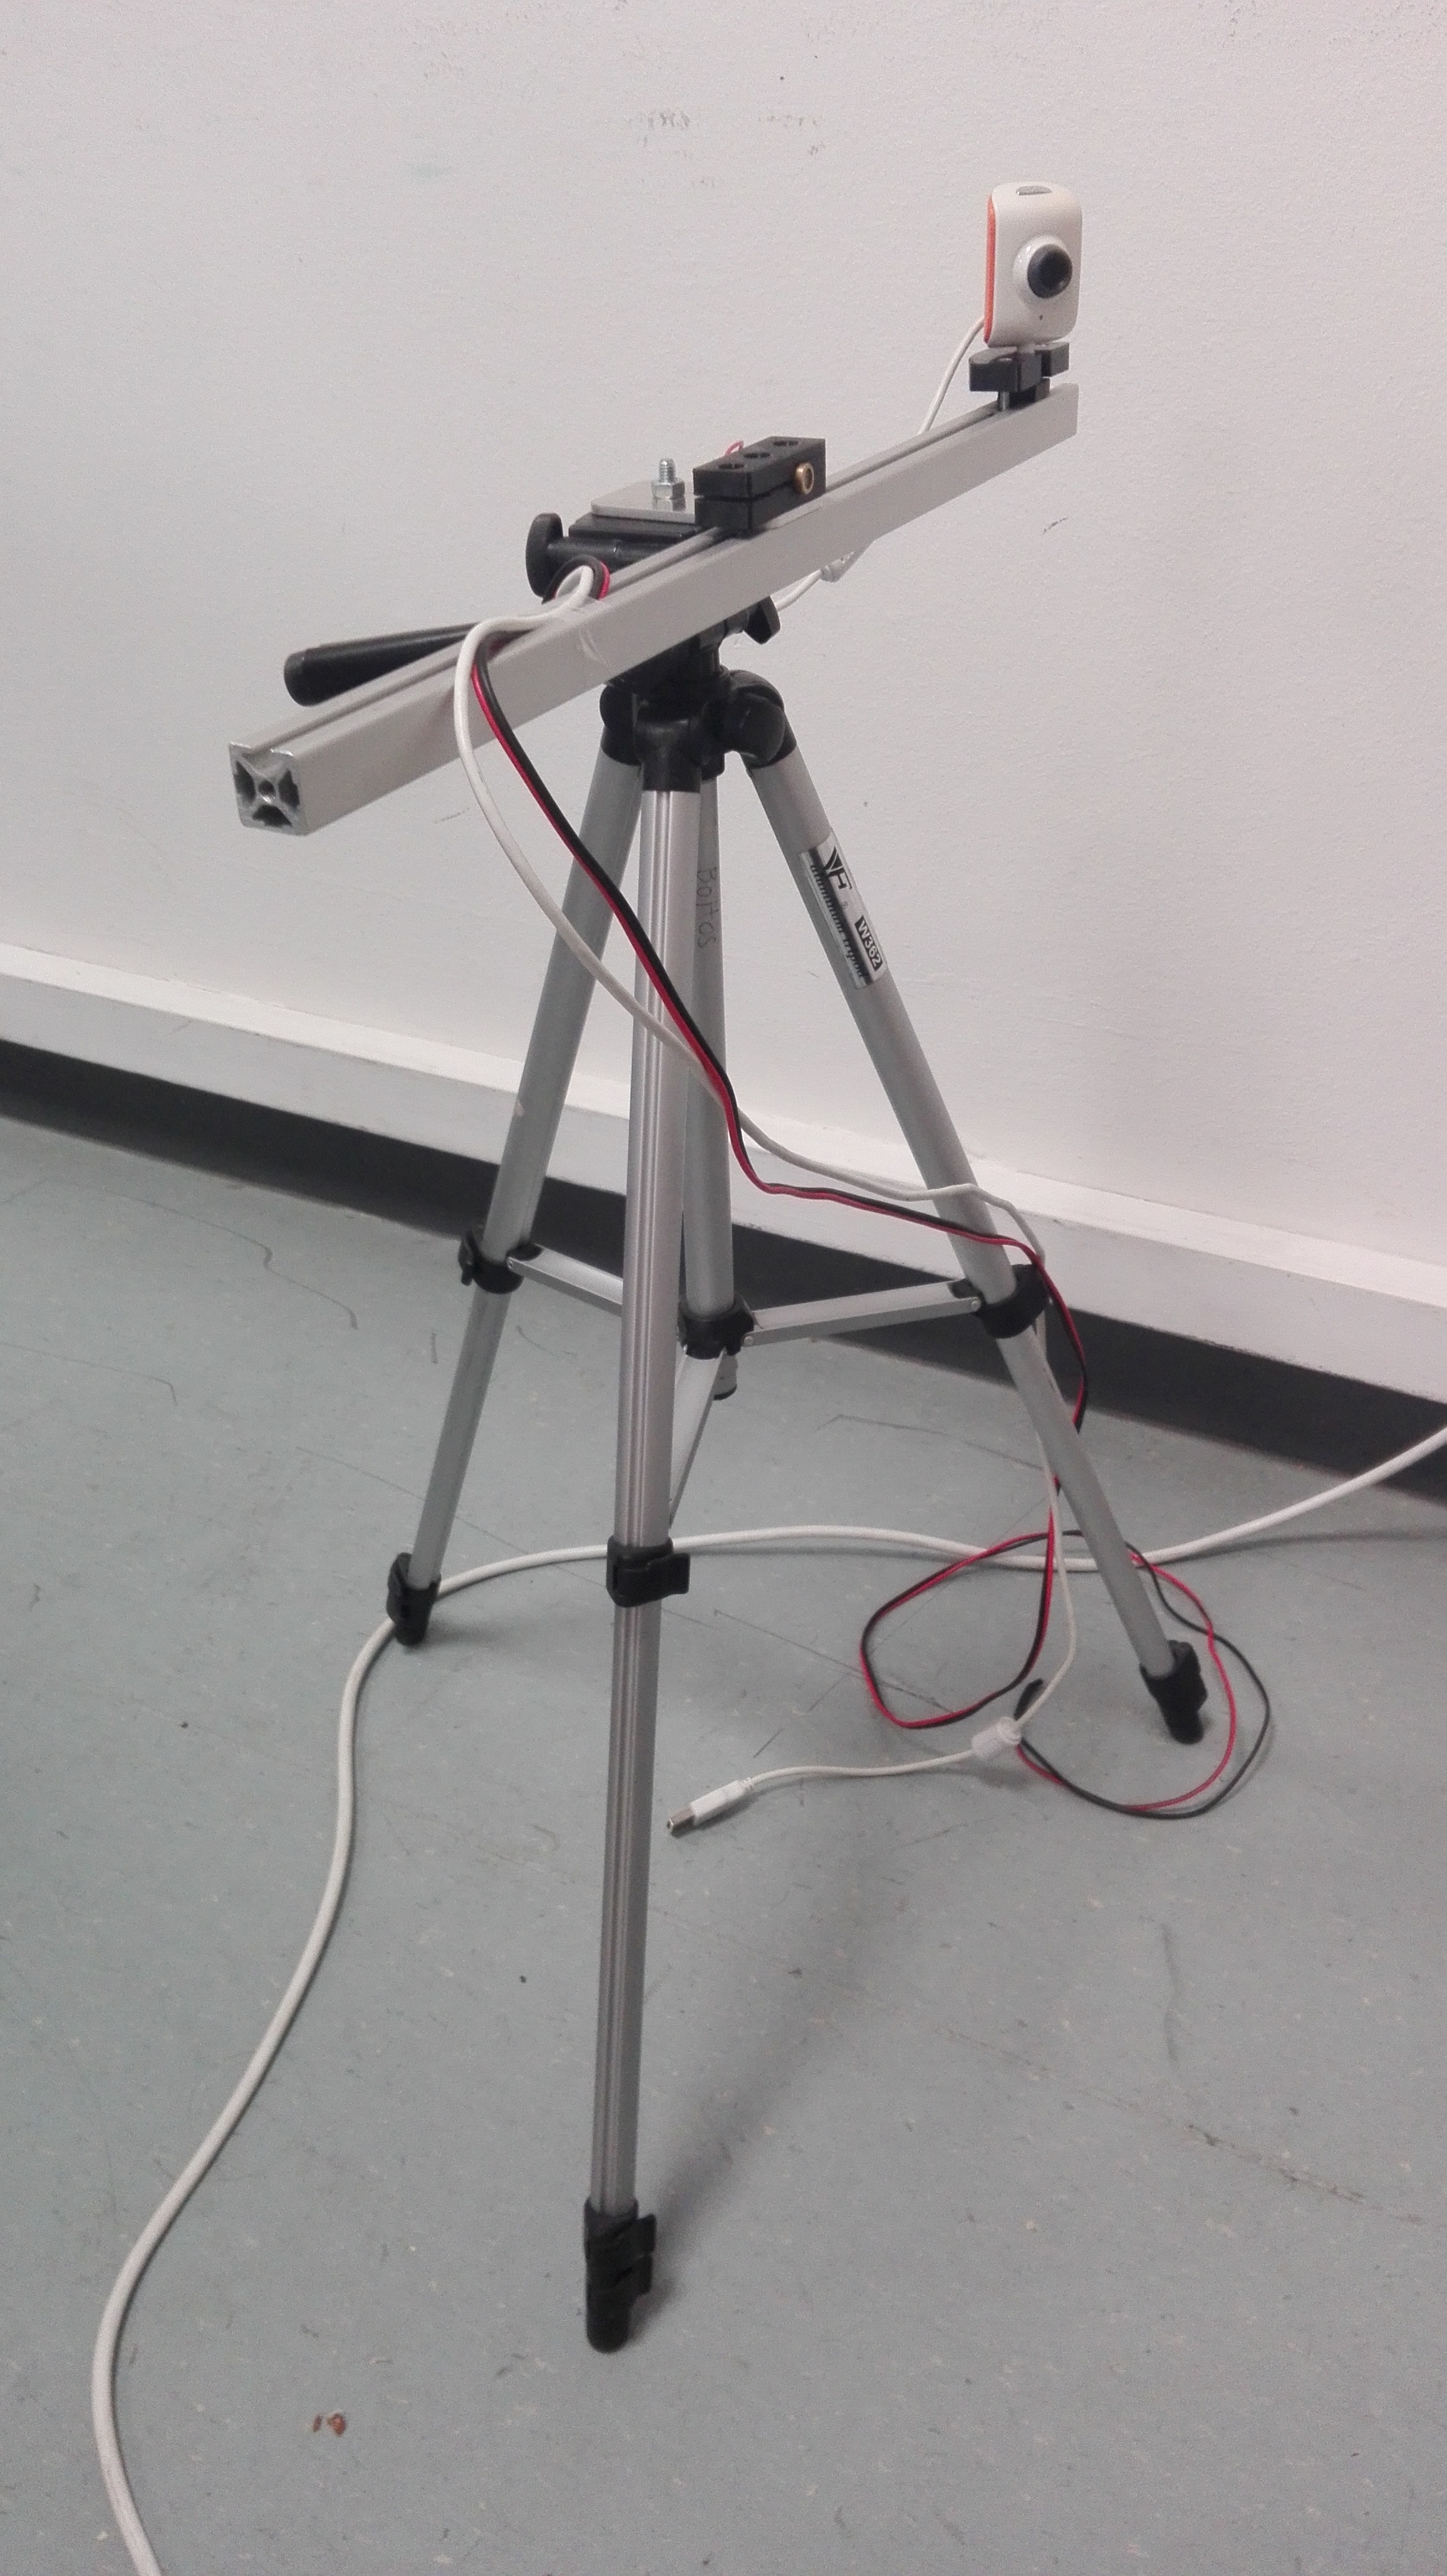
\includegraphics[width=5.5cm]{images/allvany}
	\caption{Saját készítésű eszközök}
\end{figure}
%=================================================
\section{Programkód}
Az egyes szorosan összetartozó részeket külön függvényben írtuk meg, amiket a főprogram, a scan\_object.m hív meg. A függvények csak a továbbiakban is használt változókat adják vissza, így redukáltuk a Workspace-en található vektorok számát.
\subsection{Kamera kalibráció}
\subsection{Perifériák inicializálása}
\subsection{Képek vágása}
\subsection{Transzformáció meghatározása}
\subsection{Szükséges változók deklarálása}
\subsection{Szkennelés folyamata}
\subsubsection{Lézerfény detektálása}
\subsubsection{A forgóasztal léptetése}
\subsubsection{Képek transzformációja}
\subsubsection{Pontfelhő generálása}
%=================================================
\section{Eredmények, a módszer korlátai}
%=================================================
\section{Továbbfejlesztési irányok}
%=================================================
\newpage
\begin{thebibliography}{9} 
\bibitem{feladatkiiras} 
Feladatkiírás\\
\texttt{http://mogi.bme.hu/letoltes/MECHATRONIKAI\%20\&\%20IR\%C3\%81NY\%C3\%8DT\%C3\%81\\
STECHNIKAI\%20T\%C3\%81RGYAK/MECHATRONIKA\_PROJEKT\_BMEGEFOAMM3/Feladatlapok\_M/}\\
2018.05.16.
\end{thebibliography}

\end{document}